\documentclass[tikz]{standalone}
\usepackage{amsmath, amssymb, physics, tikz}
\usetikzlibrary{decorations.pathreplacing, positioning}
\begin{document}

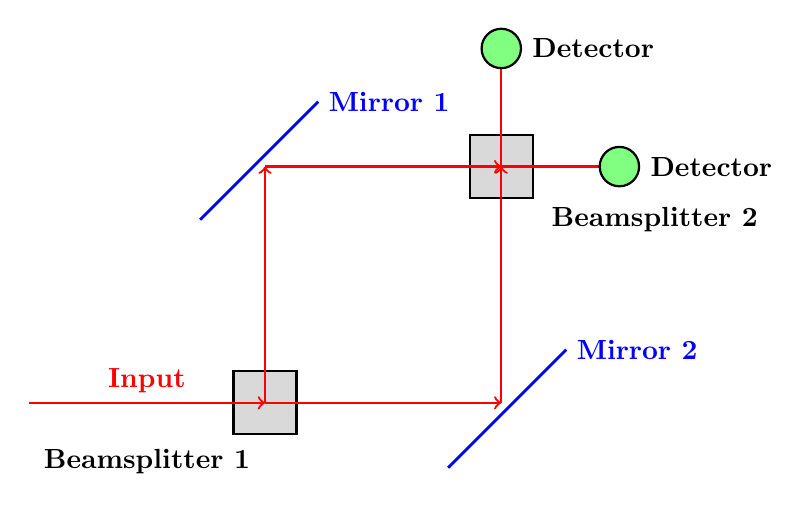
\begin{tikzpicture}[scale=1.5, thick]

    % Define styles
    \tikzstyle{mirror} = [line width=1pt, blue]
    \tikzstyle{beamsplitter} = [draw, fill=gray!30, minimum size=0.8cm]
    \tikzstyle{detector} = [draw, fill=green!50, circle, minimum size=0.5cm, label=right:\textbf{Detector}]

    % Define key points
    \coordinate (input) at (-2, 0);
    \coordinate (bs1) at (0, 0);
    \coordinate (m1) at (0, 2);
    \coordinate (m2) at (2, 0);
    \coordinate (bs2) at (2, 2);
    \coordinate (detector1) at (3, 2);
    \coordinate (detector2) at (2, 3);

    % Draw mirrors
    \draw[mirror] (-0.55, 1.55) -- (0.45, 2.55) node[right, blue] {\textbf{Mirror 1}};
    \draw[mirror] (1.55, -0.55) -- (2.55, 0.45) node[right, blue] {\textbf{Mirror 2}};

    % Draw beamsplitters
    \node[beamsplitter] at (bs1) {};
    \node[beamsplitter] at (bs2) {};

    % Draw input beam
    \draw[->, red, thick] (input) -- (bs1) node[midway, above, red] {\textbf{Input}};

    % Paths from first beam splitter
    \draw[->, red, thick] (bs1) -- (m1);
    \draw[->, red, thick] (bs1) -- (m2);

    % Reflections from mirrors
    \draw[->, red, thick] (m1) -- (bs2);
    \draw[->, red, thick] (m2) -- (bs2);

    % Paths from second beam splitter to detectors
    \draw[->, red, thick] (bs2) -- (detector1);
    \draw[->, red, thick] (bs2) -- (detector2);

    % Detectors
    \node[detector] at (detector1) {};
    \node[detector] at (detector2) {};

    % Labels
    \node at (-1, -0.5) {\textbf{Beamsplitter 1}};
    \node at (3.3, 1.55) {\textbf{Beamsplitter 2}};
    \node[right] at (detector1) {};
    \node[right] at (detector2) {};

\end{tikzpicture}

\end{document}
